\documentclass[convert]{standalone}
\usepackage{tikz}
\usetikzlibrary{cd}
\usepackage{dsfont}
\usepackage{amsmath, amsthm, amssymb}
\usepackage{adjustbox}
\usepackage{mathdots}
\usepackage{xcolor}

\newcommand\encircle[1]{%
  \tikz[baseline=(X.base)]
    \node (X) [draw, shape=circle, inner sep=0] {\strut #1};}
\begin{document}

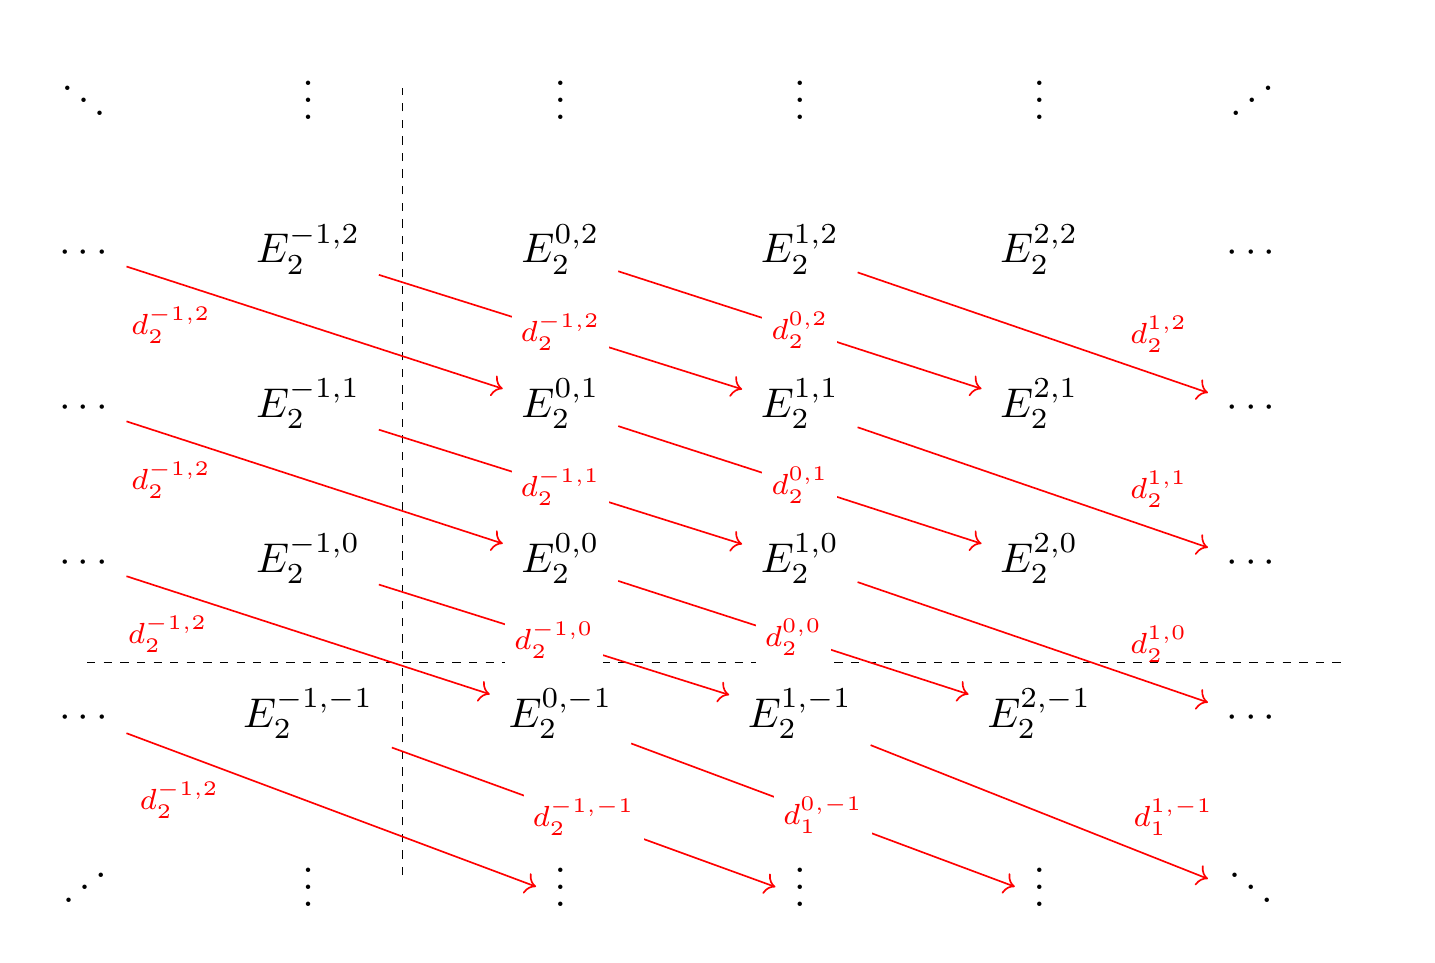
\begin{tikzpicture}
\draw [dashed] (-4,-5) -- (-4,5);
\draw [dashed] (-8, -2.3) -- (8,-2.3);
\node[scale=1.5] (a) at (0,0) {
\begin{tikzcd}[scale=4,samples=200]
\ddots  & \vdots                                  & \vdots                                 & \vdots                                & \vdots                                & \iddots \\
\cdots  \ar[red, rrd, "d_2^{-1,2}" near start, swap]& E_2^{-1,2}  \ar[red, rrd, "d_2^{-1,2}" description]  & E_2^{0,2}  \ar[red, rrd, "d_2^{0,2}" description]  & E_2^{1,2}  \ar[red, rrd, "d_2^{1,2}" near end]  & E_2^{2,2} 	& \cdots     & \\
\cdots  \ar[red, rrd, "d_2^{-1,2}" near start, swap]& E_2^{-1,1}  \ar[red, rrd, "d_2^{-1,1}" description]  & E_2^{0,1}  \ar[red, rrd, "d_2^{0,1}" description]  & E_2^{1,1}  \ar[red, rrd, "d_2^{1,1}" near end]  & E_2^{2,1}	 & \cdots     & \\
\cdots  \ar[red, rrd, "d_2^{-1,2}" near start, swap]& E_2^{-1,0}  \ar[red, rrd, "d_2^{-1,0}" description]  & E_2^{0,0}  \ar[red, rrd, "d_2^{0,0}" description]  & E_2^{1,0}  \ar[red, rrd, "d_2^{1,0}" near end]  & E_2^{2,0}	& \cdots     & \\
\cdots  \ar[red, rrd, "d_2^{-1,2}" near start, swap]& E_2^{-1,-1} \ar[red, rrd, "d_2^{-1,-1}" description] & E_2^{0,-1} \ar[red, rrd, "d_1^{0,-1}" description] & E_2^{1,-1} \ar[red, rrd, "d_1^{1,-1}" near end] & E_2^{2,-1}	 & \cdots     & \\
\iddots & \vdots     & \vdots     & \vdots     & \vdots	    & \ddots     &
\end{tikzcd}
};
\end{tikzpicture}

\end{document}
